\section{Opposite Sign Dileptons}
\label{sec:osstudies}

This section summarizes the results of the SUSY parameter space scan
in the opposite sign dilepton channel. The measurement technique is
described in detail in a previous CMS note~\cite{osnote}. The technique
utilizes a data-driven method to estimate background characterized
by the presence of two high $P_T$, isolated, opposite sign leptons,
large $\met$, and significant jet activity. This generic signature is
sensitive to many new physics scenarios such as SUSY.  For the purposes
of this note we restrict ourselves to the $ee$, $e\mu$, and $\mu\mu$
final states, {\em i.e.}, we do not consider $\tau$'s, except in the
case that the $\tau$ decays leptonically. 

As we will show in Section~\ref{sec:osyields}, for a reasonable event
selection the main background is \ttbar decays. The data-driven
background prediction is based on a suggestion by Victor
Pavlunin~\cite{victor}. The idea is that in dilepton \ttbar events
the leptons and neutrinos from $W$ decays have on average the same
$P_T$ spectrum (modulo effects of $V-A$). One can then use the {\bf
observed} \ptll $~\equiv~|\vec{P}_T(\ell_1) + \vec{P}_T(\ell_2)|$
distribution to model the sum of neutrino $P_T$'s which is identified
with $\met$. 

The statistical analysis of the expected yields uses the same tools as in the same sign analysis.

\subsection{Event Yields}
\label{sec:osyields}

The expected event yields in 100~pb$^{-1}$ after applying the event selections
described in Section~\ref{sec:eventselection} to the data sets described in
Section~\ref{sec:datasamples} are detailed below: the SM yields are listed in
Table~\ref{tab:osyields}, and the mSUGRA scan point yields are illustrated in
Fig.~\ref{fig:hobs175_100pb}.

In Fig.~\ref{fig:smvictory} one sees the SM $\met$ distribution predicted
by the data-driven background estimation technique compared with the actual 
SM $\met$ distribution. The predicted $\met$ distribution
is the $\ptll$ distribution scaled to account for the $\met>$50 GeV cut; the scale
factor is about 1.6. The predicted event yield for a given $\met$ cut is then obtained by integrating
over the $\ptll$ distribution starting from the corresponding $\ptll$ value. 
For $\met>$175 GeV, the method predicts
3.9$\pm$0.51 SM events. The true yield is 4.3$\pm$0.27 SM events, which agrees
well with the prediction. The reported errors are statistical only.

\begin{table}[hbt]
\begin{center}
\begin{tabular}{|l|c|c|c|c|}\hline
Sample           & tcMET $>$ 175   \\ \hline
$t\overline{t}$  &   3.99          \\ 
$WW$             &   0.19          \\ 
$WZ$             &   0.01          \\ 
$ZZ$             &   0.01          \\ 
$W$+jets         &   0             \\
$Z$+jets         &   0             \\ 
Single top       &   0.05          \\ \hline
\end{tabular}
\caption{Expected SM event yields in 100~pb$^{-1}$.\label{tab:osyields}}
\end{center}
\end{table}

\begin{figure}[htb]
\begin{center}
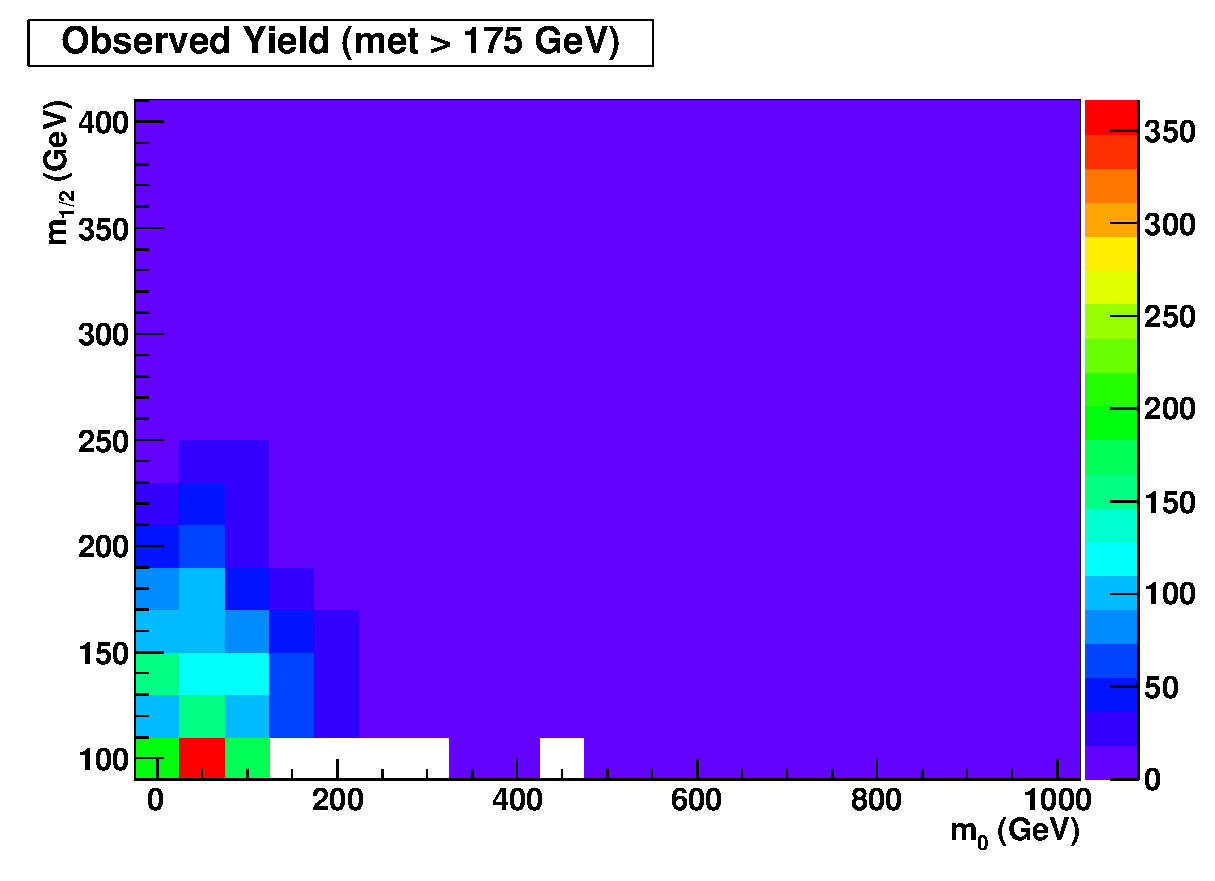
\includegraphics[width=0.7\linewidth]{figs/hobs175_100pb.eps}
\caption{Expected mSUGRA scan point event yields in 100~pb$^{-1}$\label{fig:hobs175_100pb}}
\end{center}
\end{figure}

\begin{figure}[htb]
\begin{center}
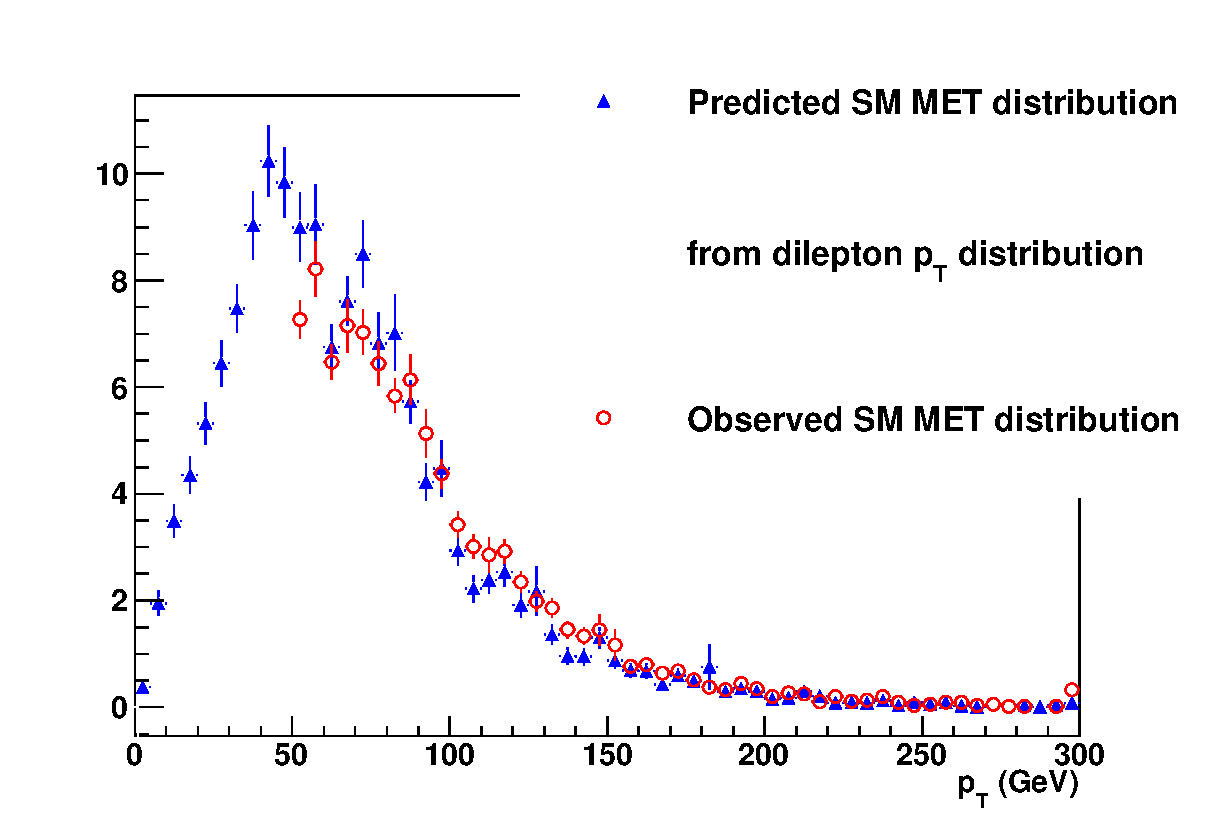
\includegraphics[width=0.7\linewidth]{figs/smvictory.eps}
\caption{Rescaled $\ptll$ distribution in the SM cocktail used to predict the $\met$ in blue, compared with the $\met$ in red.\label{fig:smvictory}}
\end{center}
\end{figure}


\subsection{Procedure for Determining $5\sigma$ Discovery Reach}
\label{sec:significance}

We  determine the  $5\sigma$  discovery reach  in the  $m_{0}-m_{1/2}$
plane by  performing our analysis at  each of the  mSUGRA scan points.
For each  point, we  determine the distributions  of $p_{T}(\ell\ell)$
and $\met$ and add these  to the corresponding SM distributions.  Then
we  perform   the  data-driven   background  estimate  by   using  the
$p_{T}(\ell\ell)$ to predict the  number of events with $\met>175$~GeV
(predicted background yield), as well  as directly count the number of
events which pass  this $\met$ cut (observed yield).   We quantify the
significance  of  the  discrepancy  between  the  observed  yield  and
predicted   background  yield   using  two   significance  estimators:
$Z_{Bi}$~\cite{cite:cousins}    and    $Z_N$~\cite{cite:conway}.   The
quantities required to calculate these estimators are:

\begin{itemize}
\item The predicted background yield
\item The relative systematic  uncertainty on the predicted background
yield (set to 25\%)
\item The  statistical uncertainty  on the predicted  background yield
($Z_N$ only, set to 0)
\item The observed yield
\end{itemize}

In   Figs.~\ref{fig:zbi} and~\ref{fig:zn} we   display  the
$Z_{Bi}$ and $Z_{N}$  significances, respectively,  assuming    integrated    luminosities   of
$100~\mathrm{pb}^{-1}$  and  $1~\mathrm{fb}^{-1}$.

\begin{figure*}[t]
\begin{center}
\begin{tabular}{c c}
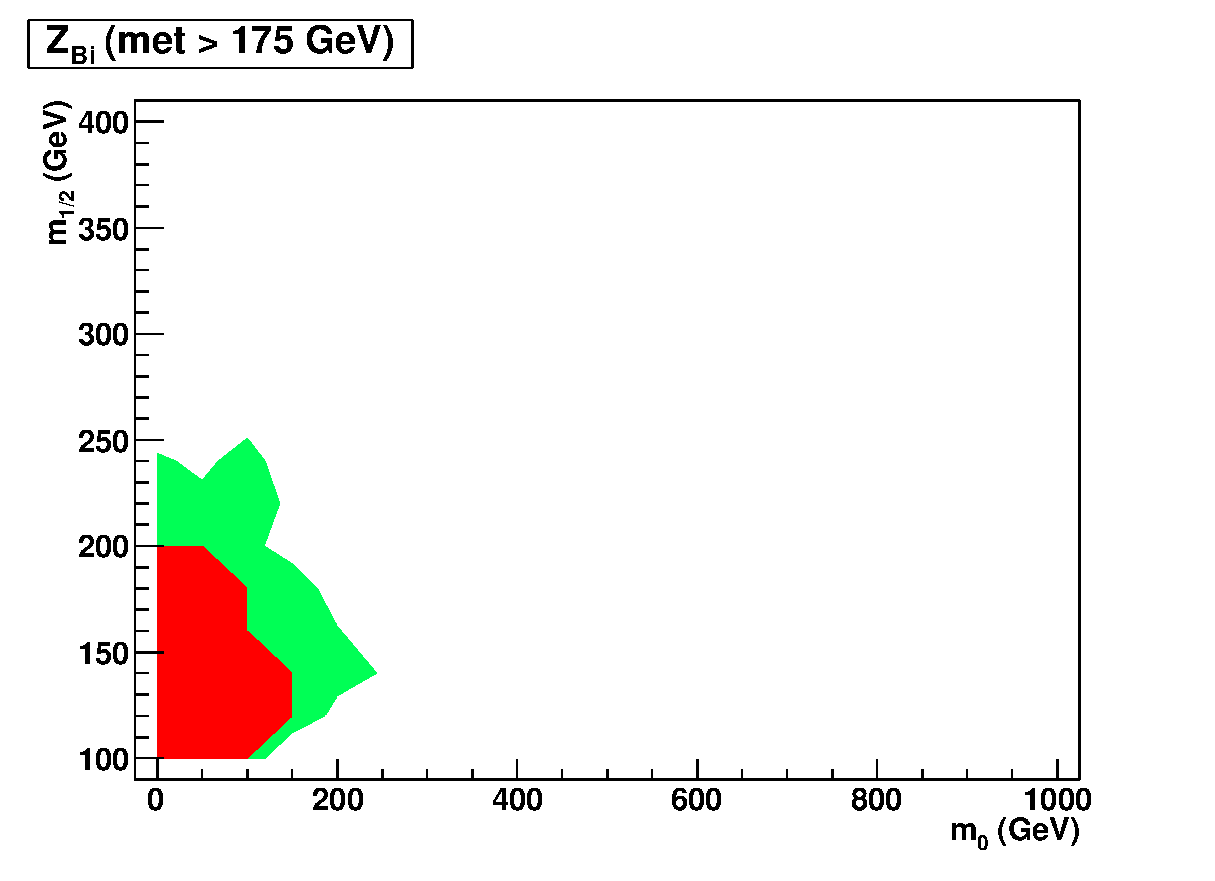
\includegraphics[height=5.5cm,clip=]{figs/hzbi175_100pb.eps}           &
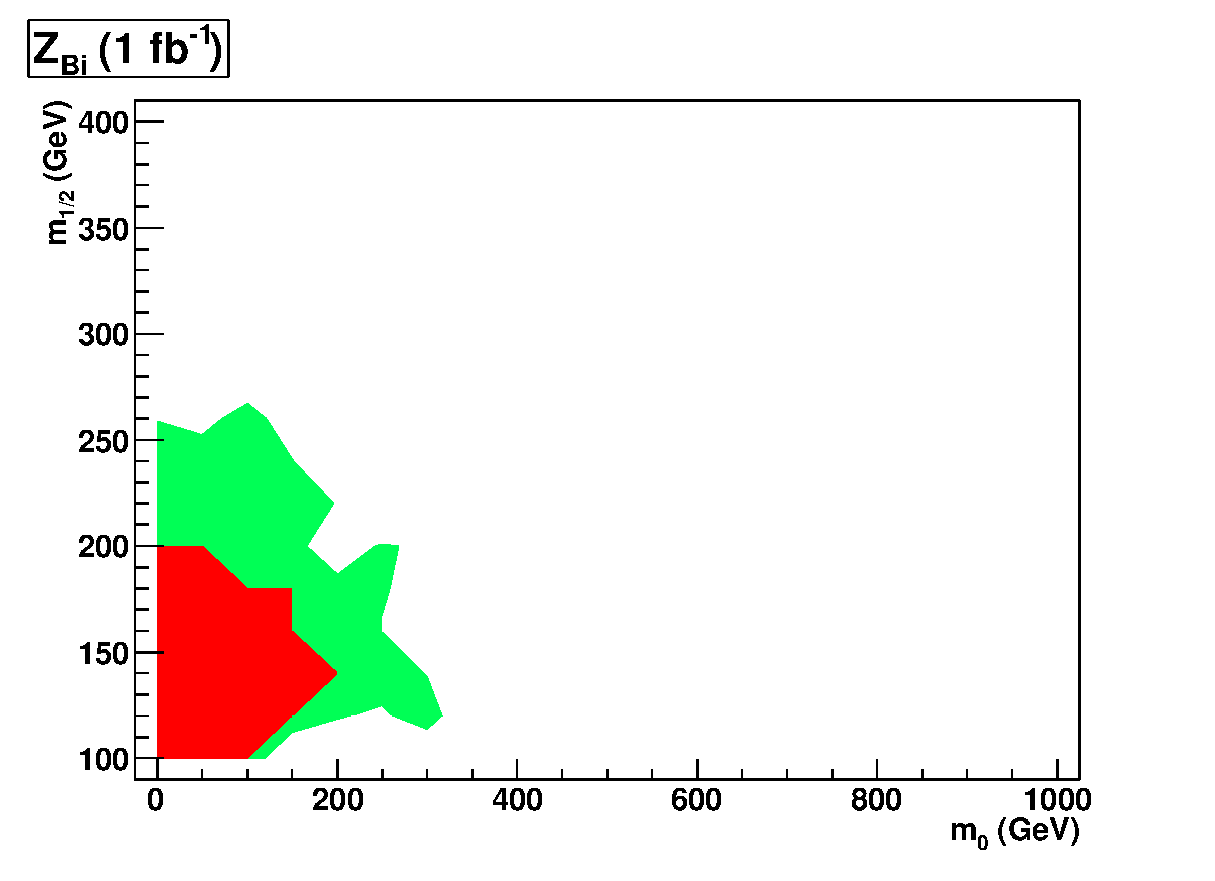
\includegraphics[height=5.5cm,clip=]{figs/hzbi175_1fb.eps}
\end{tabular}
\end{center}
\caption{The  $Z_{Bi}$  significance   in  the  $m_{0}-m_{1/2}$  plane
assuming  an  integrated  luminosity of  $100~\mathrm{pb}^{-1}$ (left)
and $1~\mathrm{fb}^{-1}$ (red). The red (green) shaded region indicates the
5$\sigma$ (3$\sigma$) sensitivity reach.   \label{fig:zbi}}
\end{figure*}

\begin{figure*}[b]
\begin{center}
\begin{tabular}{c c}
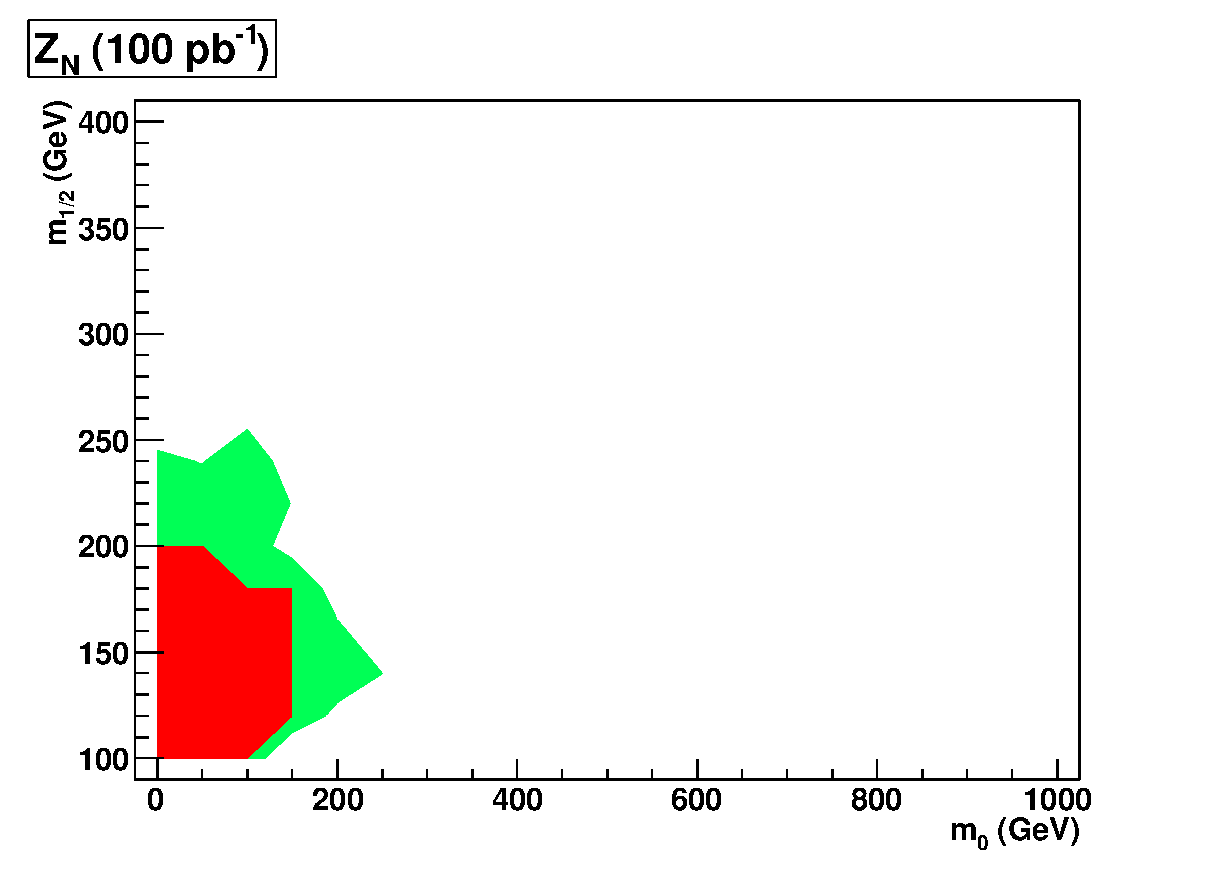
\includegraphics[height=5.5cm,clip=]{figs/hzn175_100pb.eps}           &
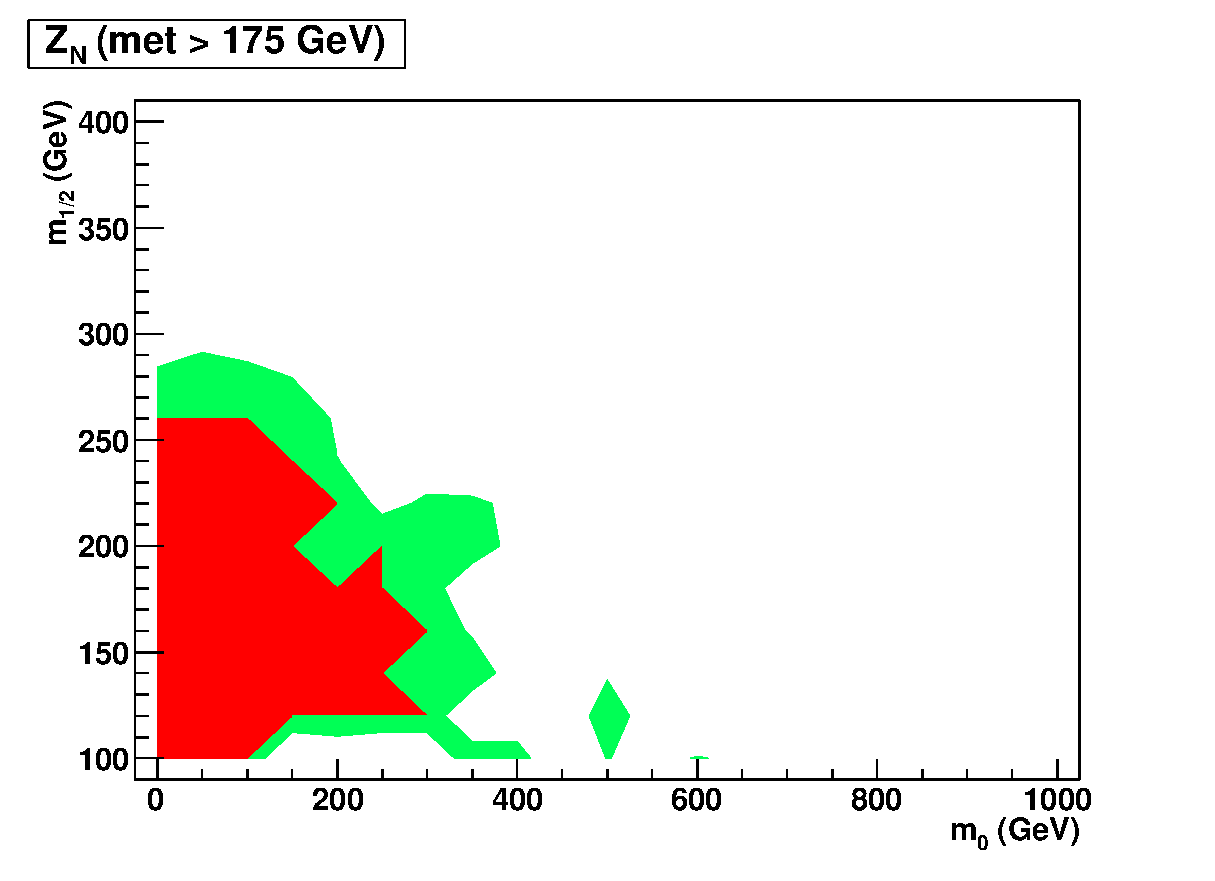
\includegraphics[height=5.5cm,clip=]{figs/hzn175_1fb.eps}
\end{tabular}
\end{center}
\caption{The  $Z_{N}$  significance   in  the  $m_{0}-m_{1/2}$  plane
assuming  an  integrated  luminosity of  $100~\mathrm{pb}^{-1}$ (left)
and $1~\mathrm{fb}^{-1}$ (red). The red (green) shaded region indicates the
5$\sigma$ (3$\sigma$) sensitivity reach.   \label{fig:zn}}
\end{figure*}


\subsection{Procedure for Excluding a Region of the mSUGRA Parameter Space}
\label{sec:exclusion}

Next we  determine the region of  the mSUGRA parameter  space which we
expect  to exclude  at 95\%  confidence level  (CL) if  we do  not see
evidence  for  signal  in data.   We  assume  that  we find  the  same
predicted background yield  and observed yield in data  that we expect
to  find based on  our SM  MC. We  use this  information to  exclude a
subset of the mSUGRA points using the following procedure.

The first  step is to  determine the 95\%  CL upper limit (UL)  on the
signal yield using a Bayesian method~\cite{bayes}. The required  inputs 
are: the observed yield, the
relative  uncertainty in  the  signal acceptance  (set  to 15\%),  the
predicted  background yield,  and  the total  error  on the  predicted
background yield. We evaluate this  error as the quadrature sum of the
systematic error (set  to 25\% of the predicted  background yield) and
the  statistical   uncertainty,  equal  to   $k\sqrt{N_{BKG}}$,  where
$k\approx1.6$ is  the scaling factor applied  to the $p_{T}(\ell\ell)$
distribution to  account for the  $\met>50~$GeV cut, and  $N_{BKG}$ is
the   predicted    background   yield.    We   find    an   error   of
$\sigma_{BKG}=3.4$     for     100~pb$^{-1}$     ($N_{BKG}=4$)     and
$\sigma_{BKG}=14.2$ for 1~fb$^{-1}$  ($N_{BKG}=40$). These values lead
to  95\% CL  ULs  of 7.6  signal  events and  33.1  signal events  for
100~pb$^{-1}$ and  1~fb$^{-1}$, respectively. It should  be noted that
bayes.f assumes a Gaussian  error distribution, while for our analysis
(especially  at 100~pb$^{-1}$ where  the background  yield is  4), our
errors are Poisson-distributed.

Next, we  wish to exclude mSUGRA  points based on the  signal yield UL
derived above.   The most obvious  way to do  so is to  exclude points
which  lead  to a  difference  between  observed  yield and  predicted
background yield  which exceeds the  UL on the signal  yield. However,
due to the effects of  signal contamination, which in our analysis can
lead to large biases in  the background prediction, one cannot rely on
this difference for exclusion. Consider an mSUGRA point which leads to
an observed yield  of 110 and a predicted background  yield of 100 for
an  integrated luminosity  of 100~pb$^{-1}$.   Since  $110-100>7.6$ we
would exclude  this point using  as our metric the  difference between
observed  and predicted  yields. However,  the  statistical difference
between these yields  is only at the $\approx1\sigma$  level and hence
this point should  not be excluded at 95\% CL. Instead,  we use as our
metric  the {\em  significance}  of the  discrepancy between  observed
yield and predicted background  yield, quantified by $Z_{Bi}$.  First,
we determine the $Z_{Bi}$ significance  corresponding to the UL on the
total yield ({\em  ie.}  the observed yield plus the  UL on the signal
yield) compared  to the predicted  background yield, again  assuming a
relative systematic  uncertainty of  25\% on the  predicted background
yield.  For  100~pb$^{-1}$ we find $Z_{Bi}=2.5$ for  an observed yield
of 4+7.6=11.6 and predicted background  of 4, while for 1~fb$^{-1}$ we
find $Z_{Bi}=2.2$ for an  observed yield of 40+33.1=73.1 and predicted
background of 40.  Finally, we  exclude those mSUGRA points which lead
to  a larger  $Z_{Bi}$  significance between  the  observed yield  and
predicted   background  yield   than   these  values,   as  shown   in
Fig.~\ref{fig:exc}   for 100~pb$^{-1}$  and
1~fb$^{-1}$.


\begin{figure*}[b]
\begin{center}
\begin{tabular}{c c}
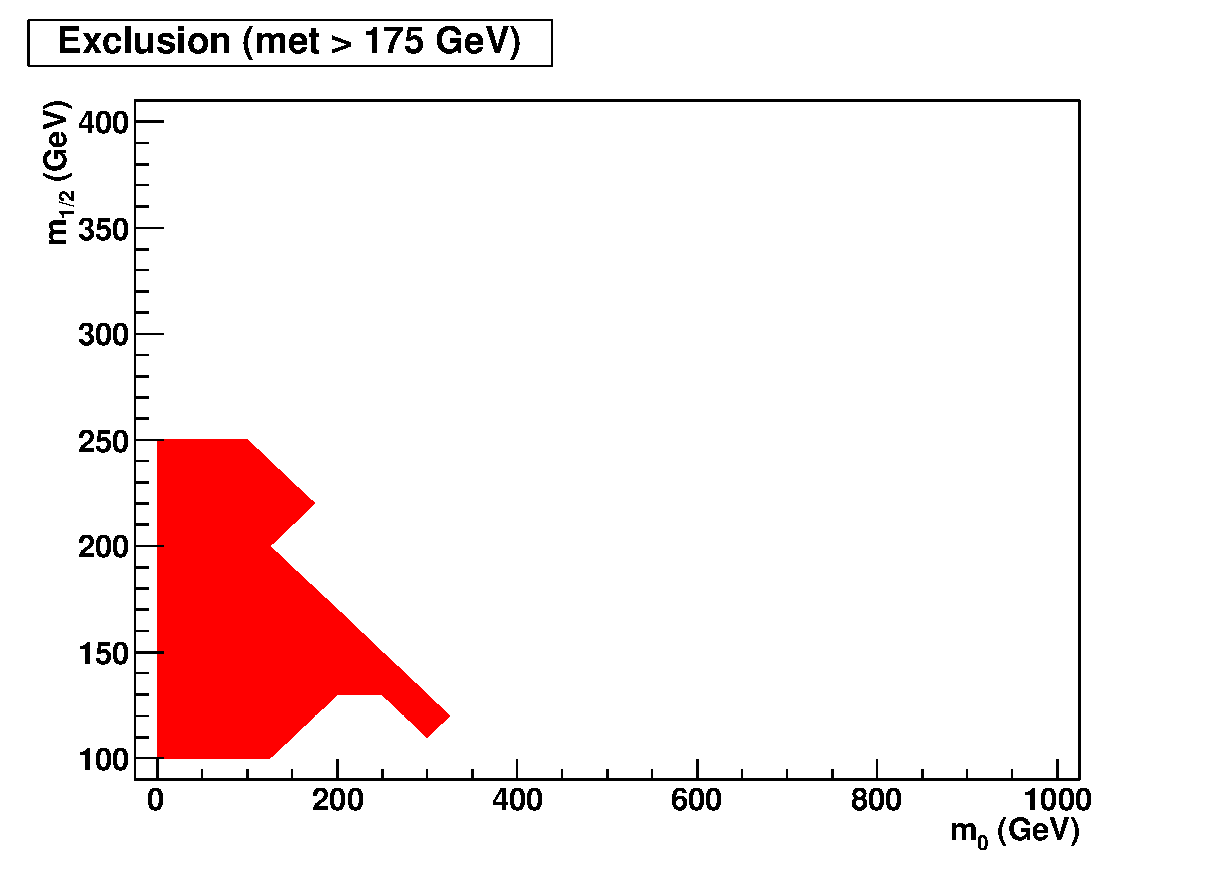
\includegraphics[height=5.5cm,clip=]{figs/hexc175_100pb.eps}           &
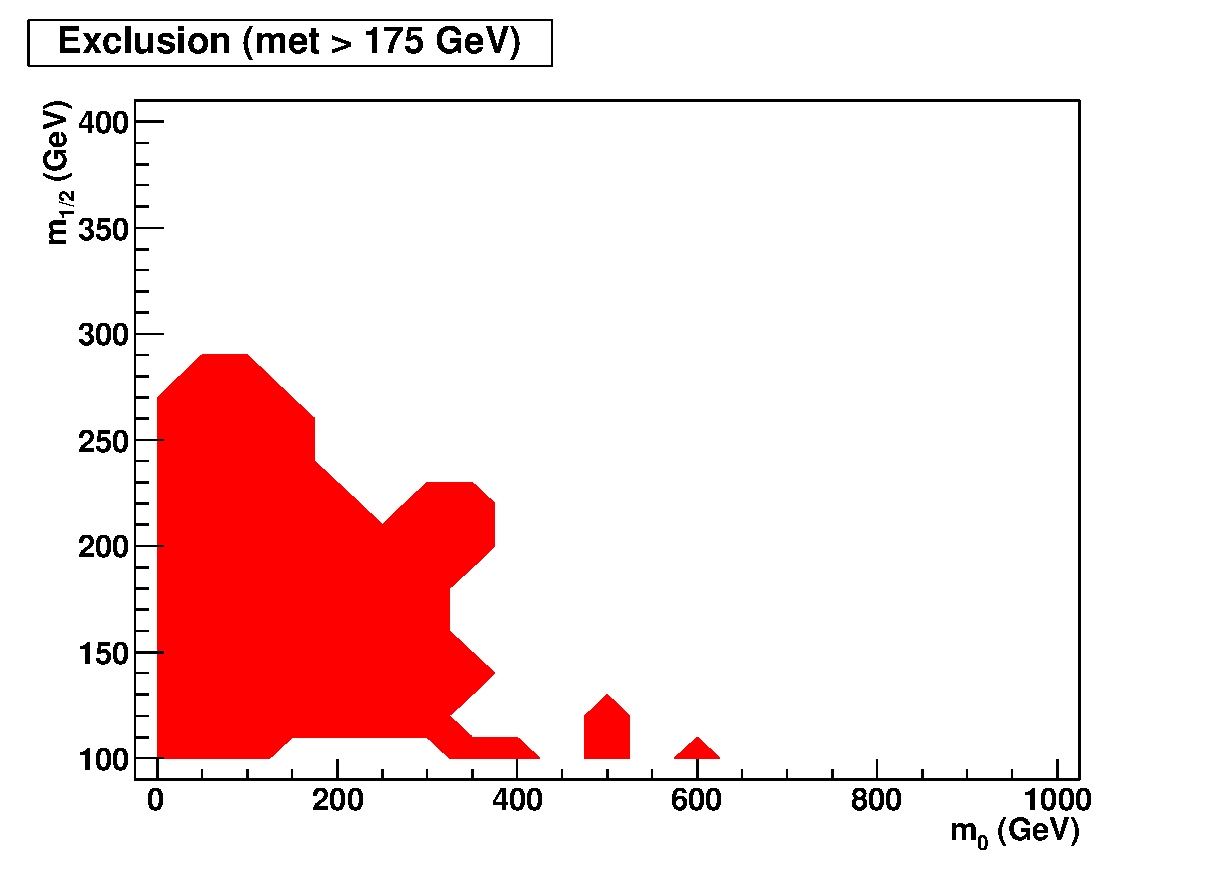
\includegraphics[height=5.5cm,clip=]{figs/hexc175_1fb.eps}
\end{tabular}
\end{center}
\caption{The excluded region (red  shaded area) of the $m_{0}-m_{1/2}$
plane       assuming      an       integrated       luminosity      of
$100~\mathrm{pb}^{-1}$ (left) and $1~\mathrm{fb}^{-1}$ (right). 
\label{fig:exc}}
\end{figure*}

